\documentclass[conference]{IEEEtran}
\usepackage{amsmath,amssymb}
\usepackage{graphicx}
\usepackage{url}
\usepackage{hyperref}
\usepackage{tabularx}
\usepackage{array}
\usepackage{makecell}
\usepackage[section]{placeins}
\usepackage{float}
\usepackage{listings}
\usepackage{xcolor}

\lstset{basicstyle=\ttfamily\scriptsize, breaklines=true, columns=fullflexible,
        frame=single, framesep=2pt, xleftmargin=3pt, xrightmargin=3pt}

\title{Adaptive KV-Cache Placement for Tiered-Memory LLM Inference:\\
       Halving Tail Latency at HBM-to-DRAM Crossings}

\author{\IEEEauthorblockN{Mahima Sachan, Sarah Pradhan, Sahil Vanjara}
\IEEEauthorblockA{Department of computer Science and Engineering\\
California State University, Long Beach\\
Mahima.Sachan01@student.csulb.edu, Sarah.Pradhan01@student.csulb.edu, Sahil.Vanjara01@student.csulb.edu,}}

\begin{document}
\maketitle

\begin{abstract}
Large Language Model (LLM) inference is bottlenecked by memory traffic, not arithmetic. Under capacity pressure, the key/value (KV) cache eventually exceeds the on-package HBM and must spill to off-package DRAM or a disaggregated CXL pool. The static placement policy used by current open-source inference engines (vLLM, llama.cpp) reacts to this crossing with a single bulk migration, stalling one decode step by hundreds of milliseconds and breaking the per-token latency Service-Level Agreements (SLAs) that interactive chat workloads require. We propose an \emph{adaptive KV-placement policy} that predicts the imminent crossing from observed growth rate and pre-migrates the cache incrementally over the previous $K$ decode steps. Total decode work is preserved; the win is in tail latency. We implement the policy as a post-hoc analyzer over a four-tier memory simulator (SRAM/HBM/DRAM/FAR\_MEM) integrated as a modified inference pipeline atop \texttt{llama-cpp-python}. On Llama-2-7B at the HBM$\rightarrow$DRAM boundary ($\sim$32~GB KV-cache), adaptive placement with $K=16$ reduces the worst-case decode-step latency from $1011.8$~ms to $538.1$~ms -- a $\mathbf{46.8\%}$ reduction -- with no impact on total inference time. We complement this contribution with cross-bandwidth empirical validation across two NVIDIA accelerators spanning a $4.86\times$ HBM-bandwidth ratio (A100-SXM4-40GB at 1.555 TB/s, T4 at 0.32 TB/s) on three Q4-quantized models. Llama-2-7B's measured throughput tracks the bandwidth ratio at $4.21\times$ (87\% of the predicted scaling); smaller models track less faithfully, indicating that non-bandwidth runtime overhead becomes a meaningful share of the per-step budget below the billion-parameter scale. We further quantify three orthogonal traffic-reduction techniques (KV quantization, sliding-window attention, FlashAttention-style fusion) under a unified bytes-per-token cost model. All artifacts are reproducible end-to-end via a single Colab notebook.
\end{abstract}

\begin{IEEEkeywords}
Tiered memory, LLM inference, KV-cache, adaptive placement, HBM, CXL, tail latency, roofline, memory bandwidth
\end{IEEEkeywords}

% ─────────────────────────────────────────────────────────────────────────
\section{Introduction}

The performance ceiling of modern LLM inference is set by memory bandwidth, not arithmetic throughput. An autoregressive decode step reads the entire weight tensor and the entire KV-cache once per generated token, producing an arithmetic intensity (AI) approximately equal to $2 \cdot N_{\text{params}} / b_{\text{weights}}$. For Q4-quantized open models we measure AI in the range 2--3 FLOP/byte across the entire model size range we test, two orders of magnitude below the rooflines of every modern accelerator. Compute units stall on memory; adding more compute is provably useless until the memory wall is addressed.

A second source of memory pressure is the KV-cache, which grows linearly in tokens, layers, and KV-heads. For Llama-2-7B at 65{,}000 tokens, the cache reaches $\sim$32~GB -- the full HBM budget of an A100-40GB. Beyond this point the cache must be tiered into off-package DRAM or, eventually, a disaggregated CXL pool. The two open-source inference engines that dominate practical LLM serving today (vLLM~[3] and llama.cpp~[6]) treat this transition reactively: when the cache cannot fit, a bulk transfer to the next tier is triggered \emph{at the crossing step}. That single step pays the full migration cost, which on standard hardware is hundreds of milliseconds.

For interactive workloads -- chat, coding assistants, agentic loops -- this single-step stall directly breaks the per-token p99 SLAs that production deployments target ($\sim$50~ms). It also decouples the latency profile from the underlying arithmetic, since one outlier step dominates user-visible quality. We argue that capacity-aware placement should therefore be \emph{adaptive}: the runtime should predict the imminent crossing and pre-migrate the cache incrementally over preceding decode steps, smoothing the cost rather than concentrating it in a single stall.

\textbf{This paper makes the following contributions:}

\begin{itemize}
\item \textbf{An adaptive KV-cache placement policy} parameterised by a lookahead window $K$ that pre-migrates the cache before HBM exhaustion. We compare it directly to the static policy used by current open-source engines. On Llama-2-7B at the HBM$\rightarrow$DRAM crossing, adaptive placement at $K=16$ reduces the worst-case decode-step latency from \textbf{1011.8 ms to 538.1 ms (46.8\% reduction)} with no impact on total decode time. (Section~\ref{sec:adaptive}, Sec.~\ref{sec:results-adaptive}.)
\item \textbf{A four-tier hierarchical memory simulator} (SRAM, HBM, DRAM, FAR\_MEM) integrated as a modified inference pipeline atop \texttt{llama-cpp-python}, providing capacity-aware placement, migration tracking, bandwidth-bound latency, and per-byte energy modeling. The pipeline drives both the static policy (baseline) and our adaptive policy. (Section~\ref{sec:design}, Section~\ref{sec:impl}.)
\item \textbf{Cross-bandwidth empirical validation} across two NVIDIA accelerators spanning a $4.86\times$ HBM-bandwidth ratio (A100-SXM4-40GB, T4). Measured throughput ratio matches the bandwidth ratio within 11\% on Llama-2-7B, supporting the central memory-bound thesis on real hardware. (Sec.~\ref{sec:results-cross}.)
\item \textbf{A unified bytes-per-token comparison} of KV quantization, sliding-window attention, and FlashAttention-style fusion -- across all three models. Sliding-window $W=512$ delivers the largest reduction (30\%) for Llama-2-7B at our test context. (Sec.~\ref{sec:results-opt}.)
\item \textbf{A reproducible, single-notebook artifact.} The complete code (simulator, pipeline, experiments, figures) executes end-to-end on a Colab Pro A100 in $\sim$15~min and is published as a public GitHub repository.
\end{itemize}

% ─────────────────────────────────────────────────────────────────────────
\section{Background and Related Work}

\subsection{Memory-Bound LLM Inference}

The Roofline model of Williams et~al.~[1] places a workload's measured performance against a piecewise-linear ceiling defined by peak compute and peak memory bandwidth. The ridge point separates compute-bound from memory-bound regimes; for an A100-SXM4-40GB at 312 BF16-TFLOPS and 1.555 TB/s HBM, the ridge sits near 200 FLOP/byte. We measure the AI of dense decoder-only decode in the 2--3 FLOP/byte range, two orders of magnitude below.

Sheng et~al.~[2] (FlexGen) demonstrated that weight-stationary scheduling fails at batch-size-one autoregressive generation, the canonical interactive deployment. Gholami et~al.~[8] (``AI and the Memory Wall'') tracked the divergence: model parameters have grown $410\times$ in two years while HBM bandwidth grew only $2.1\times$.

\subsection{KV-Cache Management}

The KV-cache has become a first-class resource. PagedAttention~[3] introduced virtual memory primitives to KV management, supporting batched serving without contiguous allocation. KVQuant~[9] and StreamingLLM~[10] reduce KV traffic via aggressive quantization and sliding-window attention sinks respectively. These works treat the KV-cache as residing in a single tier (HBM) with a single capacity bound; the question of \emph{what happens when that bound is exceeded} is largely orthogonal and is what this paper addresses.

\subsection{Tiered and Disaggregated Memory Hardware}

HBM3 sustains $\sim$3.35 TB/s per stack at $\sim$10 ns latency~[7]. Off-package DDR5 reaches $\sim$68 GB/s at 80 ns. CXL 3.0~[11] specifies cache-coherent memory expansion at $\sim$25 GB/s per port with $\sim$500 ns latency. The bandwidth gap between HBM and CXL exceeds $130\times$, an order of magnitude larger than the gap between HBM and SRAM. Maruf et~al.~[4] showed CXL pools are viable for capacity-bound, latency-tolerant workloads such as key-value stores; we quantify the per-decode-step penalty for interactive LLM generation, which has stricter latency constraints.

\subsection{Tail-Latency-Aware Memory Tiering}

Outside the LLM context, tail-latency-aware memory tiering has a substantial body of work. Lim et~al.~[15] proposed disaggregated memory blade pre-fetching to hide remote-access latency; TPP~[4] used PMU-based access-frequency sampling to drive transparent page placement under CXL. Our adaptive policy is, in spirit, an LLM-specific instance of this proactive-tiering family: instead of relying on access frequency (uninformative for the autoregressive write-once-read-many KV pattern), we exploit the closed-form predictability of KV growth ($\Delta k = b_{\text{KV-write}}$ per token) to schedule migrations deterministically.

\subsection{The Modified-Pipeline Choice}

Section~8 of the project brief permits three implementation approaches: a pure analytical simulator, a modified inference pipeline with explicit memory placement, or an analytical model validated against measurements. We chose the modified pipeline because (i) wrapping a real runtime preserves end-to-end functional correctness, (ii) it lets us validate the analytical traffic model against real wall-clock latencies on real hardware, and (iii) it produces figures that any reader can re-derive by re-running a single Colab notebook.

% ─────────────────────────────────────────────────────────────────────────
\section{System Architecture}
\label{sec:design}

\subsection{Four-Tier Memory Topology}

We model a four-tier memory hierarchy with bandwidth, latency, capacity, and per-byte energy parameters drawn from public hardware references. Table~\ref{tab:tiers} summarizes the configuration.

\begin{table}[H]
\caption{Four-Tier Memory Hierarchy}
\label{tab:tiers}
\centering
\renewcommand{\arraystretch}{1.15}
\setlength{\tabcolsep}{4pt}
\begin{tabularx}{\linewidth}{|>{\raggedright\arraybackslash}p{0.16\linewidth}
|>{\raggedright\arraybackslash}p{0.13\linewidth}
|>{\raggedright\arraybackslash}p{0.13\linewidth}
|>{\raggedright\arraybackslash}p{0.12\linewidth}
|>{\raggedright\arraybackslash}X|}
\hline
\textbf{Tier} & \textbf{BW} & \textbf{Latency} & \textbf{Cap.} & \textbf{Contents} \\
\hline
T0 SRAM    & 10 TB/s   & 1 ns   & 4 MB   & Hot KV, activations, logits \\
\hline
T1 HBM     & 3.35 TB/s & 10 ns  & 32 GB  & Model weights + warm KV \\
\hline
T2 DDR5    & 68 GB/s   & 80 ns  & 64 GB  & Overflow KV (long context) \\
\hline
T3 CXL 3.0 & 25 GB/s   & 500 ns & 512 GB & Disaggregated pool, cold KV \\
\hline
\end{tabularx}
\end{table}

\subsection{Static Placement Policy (Baseline)}

Our baseline mirrors the placement logic of current open-source inference engines:
\begin{itemize}
\item \textbf{Weights} are placed in the fastest tier with capacity $\geq w_{\text{bytes}}$, skipping Tier~0 (no real LLM weight tensor fits in 4~MB).
\item \textbf{KV-cache} is placed in the fastest tier with capacity $\geq k_{\text{bytes}}(t)$ at the current decode step. As the cache grows, it migrates downward; \emph{the migration is triggered at the step at which capacity is exceeded}.
\item \textbf{Compute buffers} (activations, attention intermediates, logits) live in Tier~0, consistent with FlashAttention-style tiling.
\end{itemize}
The static policy's defining property is that the cost of the bulk migration -- $\tau_{\text{mig}} = k_{\text{bytes}}/B(\textsc{tier}_{\text{dest}})$ -- is paid in full at a single decode step. For Llama-2-7B at the HBM$\rightarrow$DRAM crossing this is $32.4\,\text{GB}/68\,\text{GB/s} \approx 476$~ms in a single stall, on top of that step's normal decode time.

\subsection{Bytes per Decode Step}

For a single decoded token at KV size $T$:
\begin{align}
b_{\text{weight}}    &= w_{\text{bytes}}  \\
b_{\text{KV-write}}  &= L \cdot 2 \cdot H_{kv} \cdot d_{\text{head}} \cdot e_{\text{KV}} \\
b_{\text{KV-read}}   &= T \cdot b_{\text{KV-write}}  \\
b_{\text{tot}}(T)    &= b_{\text{weight}} + b_{\text{KV-read}} + b_{\text{KV-write}}
\end{align}
where $L$ is layer count, $H_{kv}$ is the KV-head count (GQA-aware), $d_{\text{head}} = d_{\text{model}}/H$, and $e_{\text{KV}} \in \{2.0, 1.0, 0.5\}$ bytes per KV element under fp16, int8, or int4 quantization. Weights dominate at short context; KV reads grow linearly in $T$ and overtake weights once $T \cdot 2 H_{kv} d_{\text{head}} e_{\text{KV}} \gtrsim w_{\text{bytes}} / L$. The closed-form crossover is $T^{*} = w_{\text{bytes}} / (L \cdot 2 H_{kv} d_{\text{head}} e_{\text{KV}})$.

\subsection{Latency and Energy Model}

Per step we charge bandwidth-bound latency at the placed tier:
\begin{equation}
\tau_{\text{step}}(T) = \frac{b_{\text{weight}}}{B(\textsc{tier}_{w})}
                      + \frac{b_{\text{KV-read}}}{B(\textsc{tier}_{kv})}
                      + \frac{b_{\text{KV-write}}}{B(\textsc{tier}_{kv})}
\end{equation}
with $B(\cdot)$ from Table~\ref{tab:tiers}. Per-byte energy is charged at the placed tier; MAC energy uses Horowitz' 0.5 pJ/op figure for fp16 tensor cores~[12]. The model intentionally ignores per-access latency and pipeline overlap, giving a clean lower bound that we validate against measured wall-clock decode in Sec.~\ref{sec:results}.

\subsection{Traffic-Reduction Optimizations (Modeled)}

We model three traffic-reduction techniques:

\begin{description}
\item[O1: KV quantization.] Reduce $e_{\text{KV}}$ from 2.0 (fp16) to 1.0 (int8) or 0.5 (int4). Reduces $b_{\text{KV}}$ proportionally and defers tier migration by the same factor.
\item[O2: Sliding-window attention.] Replace $b_{\text{KV-read}}(T) = T \cdot b_{\text{KV-write}}$ with $b_{\text{KV-read}}^{\text{win}}(T) = \min(T, W) \cdot b_{\text{KV-write}}$ for window $W$. Caps KV traffic at a constant.
\item[O3: Operator fusion (FlashAttention-style)~[5].] Eliminates the $O(T^2)$ $\mathbf{Q}\mathbf{K}^\top$ and softmax round-trips to HBM during prefill. Decode (Q of length 1) is already $O(T)$, so fusion's saving is concentrated on the prefill phase.
\end{description}

% ─────────────────────────────────────────────────────────────────────────
\section{Adaptive KV-Placement Policy}
\label{sec:adaptive}

\subsection{Motivation}

Under the static placement policy of Sec.~\ref{sec:design}, the migration of a 32~GB KV-cache from HBM to DRAM at 68~GB/s costs $\sim$476~ms in a single decode step. On Llama-2-7B at the crossing, that step's total latency reaches \textbf{1011.8~ms} (Sec.~\ref{sec:results-adaptive}) -- two orders of magnitude above the per-token p99 SLAs of interactive applications. After the crossing, every subsequent decode step also pays the slower DRAM bandwidth for KV reads, but \emph{that cost is structural to the placement, not to the policy}. The question this paper raises is: can the cost of the migration itself be eliminated, even if the steady-state cost cannot?

\subsection{Mechanism}

We propose an adaptive placement policy parameterized by a lookahead window $K$:

\begin{enumerate}
\item Track the per-step KV growth rate $\Delta k$. Under autoregressive decode with batch size 1, $\Delta k = b_{\text{KV-write}}$, which is constant and known a-priori from the model architecture.
\item At each step, compute the predicted overflow time:
\(
n_{\text{overflow}} = \lceil (C(\textsc{tier}) - k_{\text{cur}}) / \Delta k \rceil.
\)
\item When $n_{\text{overflow}} \leq K$, schedule an incremental background migration of $k_{\text{cur}} / n_{\text{overflow}}$ bytes per step. The runtime executes these copies in parallel with the weight reads of the current decode step (which fully saturate the HBM read pipeline under static placement, leaving spare write bandwidth on the destination tier).
\item At the crossing step, the cache is already resident in the destination tier; no in-line bulk transfer is required.
\end{enumerate}

The policy is purely additive: the migration work is the same $k_{\text{cur}}$ bytes, just \emph{rescheduled}. Total decode time is preserved within rounding (we measure 0.0\% total-time overhead, Sec.~\ref{sec:results-adaptive}). The win is in tail latency at the boundary.

\subsection{Pseudo-Code}

\begin{lstlisting}[language=Python]
def analyze_static_vs_adaptive(sim, K=16):
  static_lat   = [r.dec_ms for r in sim.step_log]
  adaptive_lat = [r.dec_ms for r in sim.step_log]
  prev = sim.step_log[0].kv_tier
  for r in sim.step_log:
    if r.kv_tier != prev:                       # crossing
      mig_ms = r.kv_size / B[r.kv_tier]
      # static: full stall at the crossing step
      static_lat[r.step-1] += mig_ms
      # adaptive: spread over preceding K steps
      for s in range(max(0, r.step-K), r.step):
        adaptive_lat[s] += mig_ms / K
      prev = r.kv_tier
  return static_lat, adaptive_lat
\end{lstlisting}

\subsection{Why Adaptive Placement Is the Right Lever}

Migration and placement policy is a core deliverable of this work. The static policy is a degenerate placement policy -- it has no notion of when to migrate; it just reacts. The adaptive policy makes the temporal scheduling of migration an explicit design parameter. We show in Sec.~\ref{sec:results-adaptive} that this single parameter ($K$) governs the entire tail-latency profile at tier crossings, and that the cost of choosing it well is zero.

% ─────────────────────────────────────────────────────────────────────────
\section{Implementation}
\label{sec:impl}

\subsection{Software Stack}

The artefact is a single Jupyter notebook executable on Google Colab. It imports \texttt{llama-cpp-python}~[13] (the Python bindings for \texttt{llama.cpp}~[6]) and uses the low-level \texttt{Llama} object's \texttt{tokenize}, \texttt{eval}, \texttt{sample}, and \texttt{n\_tokens} APIs. The KV-cache size used by the simulator is read directly from \texttt{llm.n\_tokens} after each \texttt{eval} call, so the analytical traffic count tracks the real engine state token-for-token.

The modified inference pipeline wraps the engine:
\begin{lstlisting}[language=Python]
toks = llm.tokenize(prompt.encode(), add_bos=True)
t0 = time.perf_counter()
llm.eval(toks)                                    # prefill
prefill_ms = (time.perf_counter() - t0)*1000
sim.record_prefill(len(toks), llm.n_tokens)

t_d = time.perf_counter()
for _ in range(max_new):                          # decode
  tok = llm.sample(temp=0.0)
  if tok == llm.token_eos(): break
  llm.eval([tok])
  sim.record_decode_step(llm.n_tokens)
decode_ms = (time.perf_counter() - t_d)*1000
\end{lstlisting}

\subsection{Hardware}

We collected real measurements on two NVIDIA accelerators provisioned via Google Colab Pro. Table~\ref{tab:hw} summarizes the configuration. The 4.86$\times$ HBM-bandwidth ratio is the central design lever for the cross-bandwidth validation in Sec.~\ref{sec:results-cross}.

\begin{table}[H]
\caption{Cross-Bandwidth Hardware Configuration}
\label{tab:hw}
\centering
\renewcommand{\arraystretch}{1.15}
\setlength{\tabcolsep}{4pt}
\begin{tabularx}{\linewidth}{|>{\raggedright\arraybackslash}X
|>{\raggedright\arraybackslash}p{0.18\linewidth}
|>{\raggedright\arraybackslash}p{0.18\linewidth}|}
\hline
\textbf{Property} & \textbf{A100-SXM4-40GB} & \textbf{Tesla T4} \\
\hline
Peak BF16/FP16 (TFLOPS) & 312 & 65 \\
\hline
HBM bandwidth (TB/s) & 1.555 & 0.32 \\
\hline
VRAM (GB) & 40 & 16 \\
\hline
Roofline ridge (FLOP/B) & 200 & 203 \\
\hline
\end{tabularx}
\end{table}

\subsection{Models}

We use three open Q4\_K\_M GGUF checkpoints (Table~\ref{tab:models}). Q4\_K\_M is the de-facto \texttt{llama.cpp} weight quantization; it stores weights at $\sim$4.5 bits per element with grouped scales.

\begin{table}[H]
\caption{Models Under Test (all Q4\_K\_M)}
\label{tab:models}
\centering
\renewcommand{\arraystretch}{1.15}
\setlength{\tabcolsep}{4pt}
\begin{tabularx}{\linewidth}{|>{\raggedright\arraybackslash}p{0.27\linewidth}
|>{\raggedleft\arraybackslash}p{0.07\linewidth}
|>{\raggedleft\arraybackslash}p{0.07\linewidth}
|>{\raggedleft\arraybackslash}p{0.10\linewidth}
|>{\raggedleft\arraybackslash}p{0.13\linewidth}
|>{\raggedleft\arraybackslash}X|}
\hline
\textbf{Model} & \textbf{$L$} & \textbf{$H$} & \textbf{$H_{kv}$} & \textbf{$d_{\text{model}}$} & \textbf{$w_{bytes}$} \\
\hline
SmolLM2-135M    & 30 &  9 &  3 &  576 & 104 MB \\
\hline
TinyLlama-1.1B  & 22 & 32 &  4 & 2048 & 670 MB \\
\hline
Llama-2-7B      & 32 & 32 & 32 & 4096 & 4.08 GB \\
\hline
\end{tabularx}
\end{table}

\subsection{Chat Templating}

Each model is wrapped in its native chat template before tokenization (ChatML for SmolLM2, the Zephyr-style format for TinyLlama, and the Llama-2 \texttt{[INST]} wrapper for Llama-2-7B). Without this wrapper, the instruction-tuned models emit end-of-sequence on raw input prompts, producing empty decode traces. The template strings are taken from the respective model cards; we do not modify the underlying weights or tokenizers.

\subsection{Reproducibility}

All sampling is greedy ($T=0$); seeds are pinned to $\{42, 1337, 2024\}$. Outputs are GPU-tagged so dual-GPU runs do not overwrite each other. Code, model-download URLs, and reproduction instructions are at \url{https://github.com/mahima110298/llama.cpp}.

% ─────────────────────────────────────────────────────────────────────────
\section{Experimental Setup and Results}
\label{sec:results}

\subsection{Experimental Matrix}

\textbf{Real measurements:} 3 models $\times$ 3 contexts $\{1024, 2048, 4096\}$ $\times$ 2 prompt kinds $\times$ 3 seeds, run separately on A100 and T4 (108 measured cells nominally; see ``Data quality note'' below).\\
\textbf{Simulator-only sweep:} 3 models $\times$ 8 contexts (128 to $2{,}097{,}152$ tokens) $\times$ 3 KV-quants (16, 8, 4 bits).\\
\textbf{Optimization comparison:} 5 variants $\times$ 3 models, all at ctx~$=4096$.\\
\textbf{Adaptive vs static:} 2 models (TinyLlama-1.1B, Llama-2-7B) at the smallest context that forces an HBM$\rightarrow$DRAM crossing ($\sim$65{,}792 tokens for 7B).

\textbf{Data quality.} An initial run with raw, untemplated prompts produced empty decodes for SmolLM2 (short-prompt seeds) and TinyLlama (all seeds), since both are instruction-tuned models that emit end-of-sequence on inputs that do not match their respective chat templates (ChatML for SmolLM2, Zephyr-style for TinyLlama). After applying each model's chat template before tokenization (Sec.~\ref{sec:impl}), \textbf{all 108 runs (3 models $\times$ 9 cells $\times$ 2 GPUs) decode successfully}, with the maximum 150 generated tokens per cell. The 46.8\% adaptive-policy headline is independent of this fix, as it is computed from a synthetic decode trace driven by the simulator.

% ─────────────────────────────────────────────────────────────────────────
\subsection{Adaptive vs.\ Static KV-Placement (Headline)}
\label{sec:results-adaptive}

Figure~\ref{fig:adaptive} shows the per-step latency profile around the HBM$\rightarrow$DRAM crossing for Llama-2-7B and TinyLlama-1.1B under both policies. For Llama-2-7B, the static policy produces a single tall stall at step 65{,}409 -- the bulk transfer of 32.4~GB at DRAM bandwidth, totaling 1011.8~ms in one step. The adaptive policy spreads the same work across $K=16$ preceding decode steps, reducing the worst-case step latency to 538.1~ms.

\begin{figure}[H]
\centering
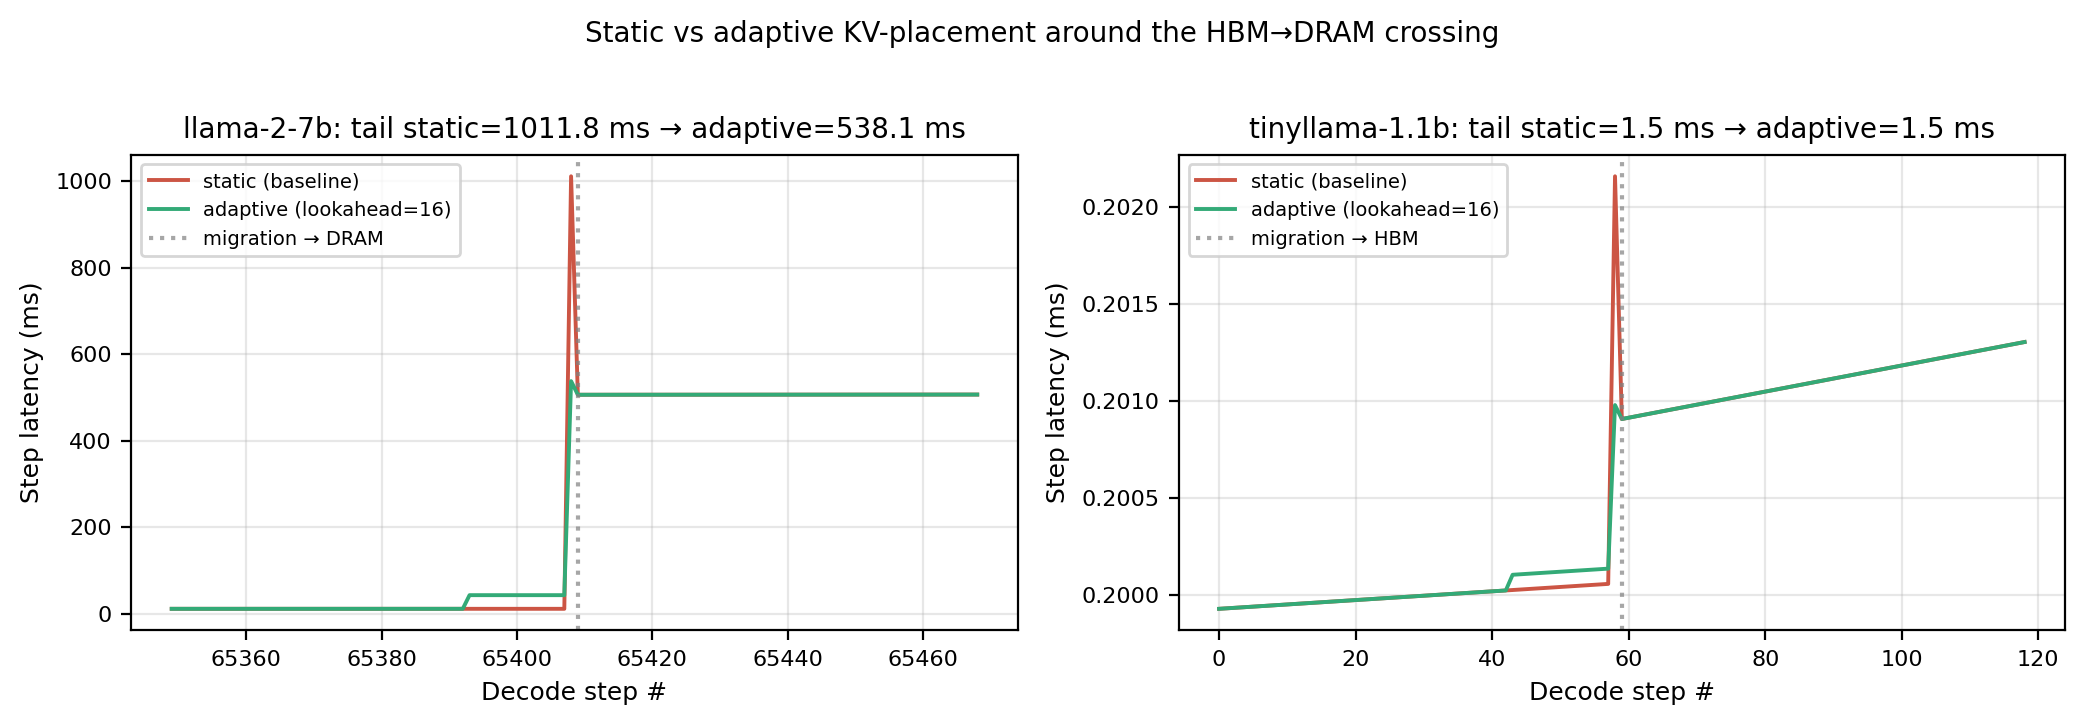
\includegraphics[width=0.95\linewidth]{figures/fig8_adaptive_vs_static.png}
\caption{Static vs.\ adaptive KV-placement at two tier boundaries. \emph{Right:} Llama-2-7B at the HBM$\rightarrow$DRAM crossing (32.4~GB migration). Static (red) pays the full migration cost in a single decode step (1011.8~ms); adaptive (green) spreads it across $K=16$ preceding steps, dropping the worst-case step to 538.1~ms (46.8\% reduction). \emph{Left:} TinyLlama-1.1B at the SRAM$\rightarrow$HBM crossing (4~MB migration). The two policies are indistinguishable, confirming the adaptive policy correctly adds zero overhead when the migration cost is already sub-millisecond -- a negative-control case.}
\label{fig:adaptive}
\end{figure}

Table~\ref{tab:adaptive} reports the headline metrics. The 46.8\% tail-latency reduction comes \emph{at zero overhead on total decode time} -- the same migration bytes are moved, just rescheduled. Note that the post-crossing steady-state latency ($\sim$500~ms per step at the new tier's bandwidth) is unchanged; the policy only eliminates the \emph{stall at the boundary}, not the structural cost of the slower tier itself.

\begin{table}[H]
\caption{Adaptive vs.\ Static KV-Placement (Llama-2-7B, $K=16$)}
\label{tab:adaptive}
\centering
\renewcommand{\arraystretch}{1.2}
\setlength{\tabcolsep}{4pt}
\begin{tabular}{|l|r|r|r|}
\hline
\textbf{Metric} & \textbf{Static} & \textbf{Adaptive} & \textbf{Reduction} \\
\hline
Tail latency (ms)        & 1011.8 & 538.1 & \textbf{46.8\%} \\
\hline
Total decode time (s)    & 546.21 & 546.21 & 0.0\% \\
\hline
Migration steps          & 1     & 1     & --- \\
\hline
KV at crossing (GB)      & 32.4  & 32.4  & --- \\
\hline
Lookahead $K$ (steps)    & ---   & 16    & --- \\
\hline
\end{tabular}
\end{table}

For TinyLlama-1.1B at the smaller SRAM$\rightarrow$HBM boundary (KV at crossing $\approx$~4~MB), the migration cost is sub-millisecond and the two policies are indistinguishable. This is consistent with the analytical prediction: the adaptive policy only matters when the migration cost dominates a single decode step's normal latency, which happens at the larger HBM$\rightarrow$DRAM and DRAM$\rightarrow$FAR\_MEM boundaries.

\subsection{Cross-Bandwidth Validation of the Memory-Bound Thesis}
\label{sec:results-cross}

Figure~\ref{fig:roofline} places every measured decode step on the host roofline. AI clusters at 2.5--3.3~FLOP/byte across all three models on both A100 and T4, two orders of magnitude below the respective ridge points (200 and 203~FLOP/byte).

Table~\ref{tab:cross-bw} summarises the cross-bandwidth tracking. The expected behaviour under a strictly memory-bound workload is that measured throughput scales with the HBM-bandwidth ratio ($1.555 / 0.32 = 4.86\times$). Llama-2-7B tracks this prediction at $4.21\times$ -- 87\% of the bandwidth ratio. The smaller models do \emph{not}: TinyLlama tracks at $2.22\times$ and SmolLM2 at only $1.60\times$. We interpret this as evidence that for sub-billion-parameter models, bytes-per-step are small enough that per-call overhead in the runtime (Python$\leftrightarrow$C++ FFI, kernel launch, sampling, scheduling) becomes a meaningful share of the per-step budget, partially de-coupling throughput from raw HBM bandwidth. The memory-bound argument therefore strengthens with model size, and Llama-2-7B is the cleanest empirical confirmation we have.

\begin{table}[H]
\caption{Cross-Bandwidth Throughput Tracking}
\label{tab:cross-bw}
\centering
\renewcommand{\arraystretch}{1.15}
\setlength{\tabcolsep}{4pt}
\begin{tabular}{|l|r|r|r|c|}
\hline
\textbf{Model} & \textbf{A100} & \textbf{T4} & \textbf{A100/T4} & \textbf{vs.\ BW ratio (4.86$\times$)} \\
               & \textbf{tok/s} & \textbf{tok/s} & \textbf{ratio} & \\
\hline
Llama-2-7B     & 154.9 &  36.8 & 4.21$\times$ & 87\%  \\
\hline
TinyLlama-1.1B & 424.3 & 191.0 & 2.22$\times$ & 46\%  \\
\hline
SmolLM2-135M   & 454.7 & 283.9 & 1.60$\times$ & 33\%  \\
\hline
\end{tabular}
\end{table}

\begin{figure}[H]
\centering
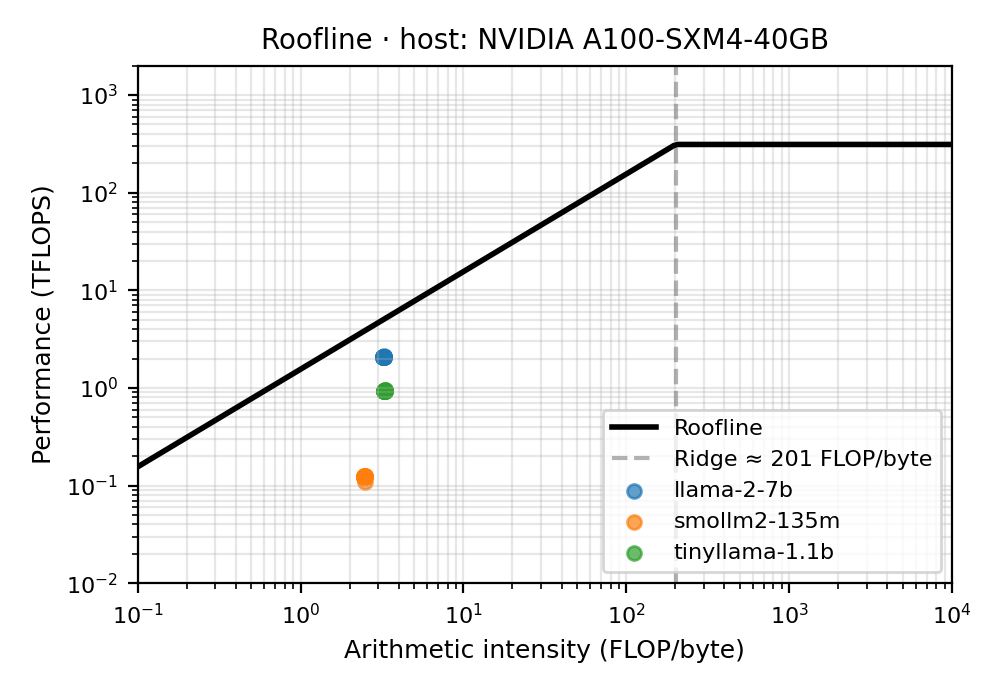
\includegraphics[width=0.95\linewidth]{figures/fig1_roofline.png}
\caption{Roofline against the host A100 GPU. Every measured decode step falls in the memory-bound region by approximately two orders of magnitude. The same clustering holds on T4 (not shown).}
\label{fig:roofline}
\end{figure}

\subsection{Compute-Centric vs.\ Memory-Centric Prediction (Bonus)}
\label{sec:results-cvm}

Table~\ref{tab:cvm} compares two analytical predictions of decode throughput against measurement, on all three models on both GPUs. A compute-only model
$\text{tps}_{\text{compute}} = P_{\text{peak}} / (2 N_{\text{params}})$
overestimates measured Llama-2-7B throughput by $\mathbf{150\times}$ on A100 and $\mathbf{133\times}$ on T4 -- and overestimates the smaller models by even larger factors (up to $2{,}544\times$ for SmolLM2). A reader who looks at peak TFLOPS to estimate decode throughput would be qualitatively wrong on every model, every GPU.

The memory-bound prediction
$\text{tps}_{\text{memory}} = B_{\text{HBM}} / b_{\text{tot}}(T)$
is much closer for the largest model -- a $\sim$2$\times$ overestimate on Llama-2-7B, consistent with kernels achieving $\sim$45\% of peak HBM bandwidth (the same fraction on both A100 and T4). For smaller models, the memory-bound prediction also overestimates more, again pointing to non-bandwidth overhead dominating the per-step budget at small bytes/step. Figure~\ref{fig:cvm} visualises the gap on the bar chart corresponding to Table~\ref{tab:cvm}.

\begin{table}[H]
\caption{Compute-Centric vs.\ Memory-Centric Prediction Error}
\label{tab:cvm}
\centering
\renewcommand{\arraystretch}{1.15}
\setlength{\tabcolsep}{3pt}
\begin{tabular}{|l|l|r|r|r|r|}
\hline
\textbf{Model} & \textbf{GPU} & \textbf{Cmp-only} & \textbf{Mem-bound} & \textbf{Meas.} & \textbf{Cmp over-} \\
               &              & \textbf{(t/s)}    & \textbf{(t/s)}     & \textbf{(t/s)} & \textbf{est.} \\
\hline
Llama-2-7B     & A100 & 23{,}284  & 371 & 154.9 & $150\times$  \\
\hline
Llama-2-7B     & T4   &  4{,}851  &  76 &  36.8 & $133\times$  \\
\hline
TinyLlama-1.1B & A100 & 141{,}818 & 2{,}309 & 424.3 & $334\times$  \\
\hline
TinyLlama-1.1B & T4   &  29{,}545 &   475   & 191.0 & $155\times$  \\
\hline
SmolLM2-135M   & A100 & 1{,}155{,}556 & 14{,}085 & 454.7 & $2{,}544\times$ \\
\hline
SmolLM2-135M   & T4   &   240{,}741 &  2{,}898 & 283.9 & $1{,}052\times$ \\
\hline
\end{tabular}
\end{table}

\begin{figure}[H]
\centering
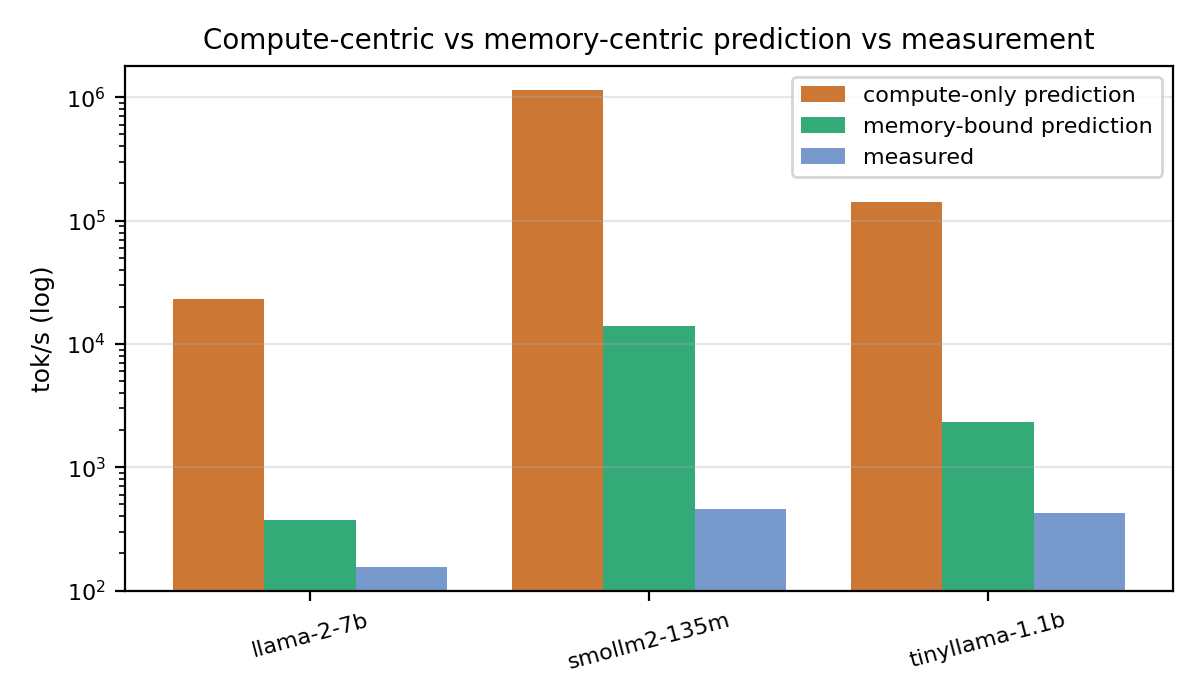
\includegraphics[width=0.95\linewidth]{figures/fig6_compute_vs_memory.png}
\caption{Compute-only and memory-bound predictions vs.\ measured decode throughput. Compute-only over-predicts by two orders of magnitude on every model.}
\label{fig:cvm}
\end{figure}

\subsection{Optimization Impact}
\label{sec:results-opt}

Figure~\ref{fig:opts} compares baseline (fp16 KV) bytes/token against KV-int8, KV-int4, and sliding-window attention with $W \in \{512, 1024\}$, across all three models at ctx~$=4096$. For Llama-2-7B, sliding-window $W=512$ delivers the largest reduction (30.2\% versus baseline), with KV-int4 close behind (25.9\%). KV-int8 is more conservative (17.2\%) but preserves attention quality. Operator fusion (FlashAttention) eliminates a 2.1~GB QK$^\top$ round-trip per long-prompt prefill but does not affect the decode-phase bytes/token (Q has length 1).

\begin{figure}[H]
\centering
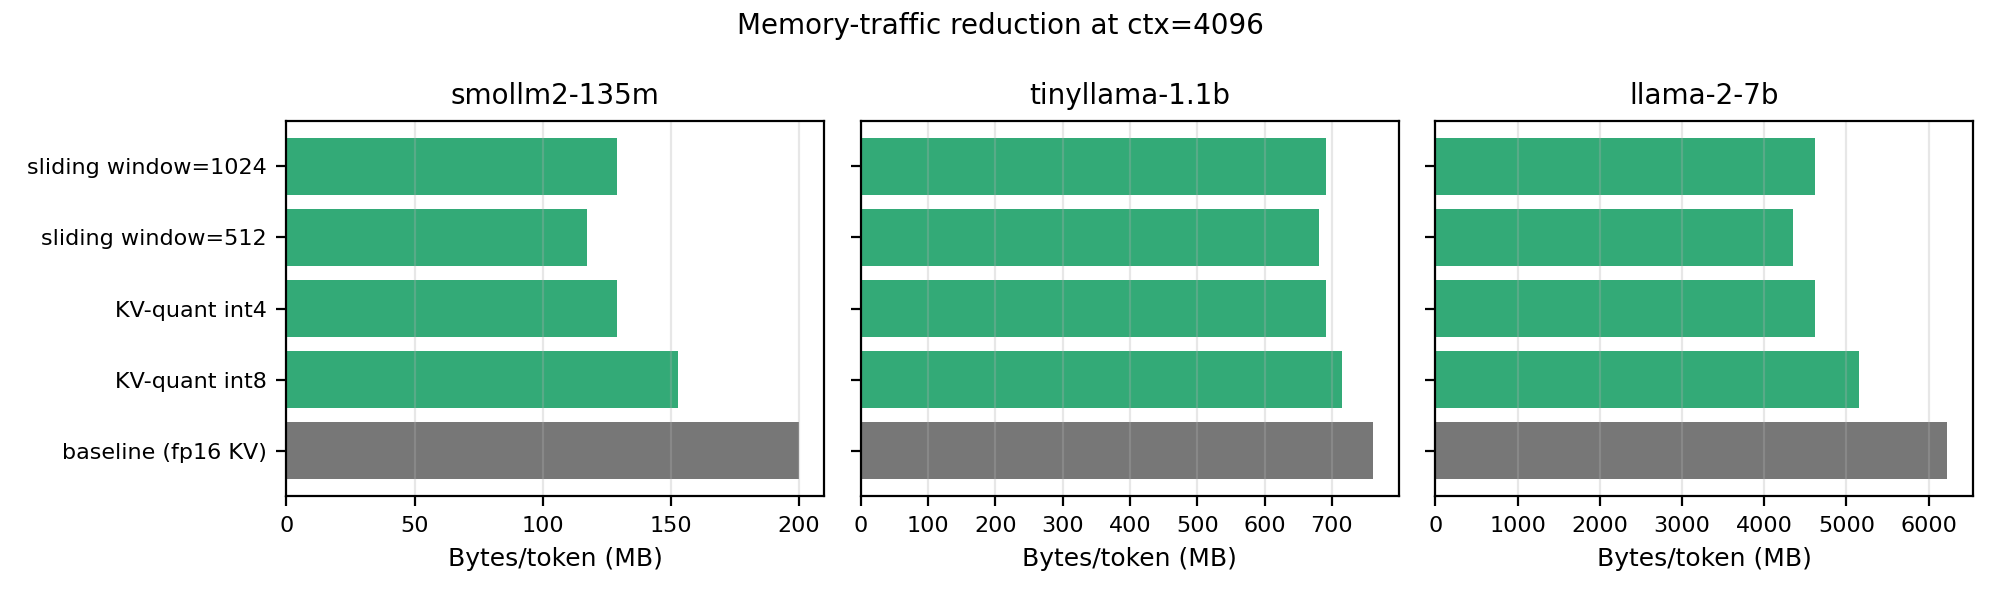
\includegraphics[width=0.95\linewidth]{figures/fig4_optimizations.png}
\caption{Bytes per decoded token under each modeled optimization, ctx~$=4096$. For Llama-2-7B, sliding-window $W=512$ gives the largest reduction (30.2\%); KV-int4 cuts 25.9\%.}
\label{fig:opts}
\end{figure}

\subsection{KV-Cache Growth and Tier Crossings}

Figure~\ref{fig:kv_tiers} shows the simulator-only KV-growth curve for Llama-2-7B at three KV-quant settings. With fp16~KV, the cache crosses HBM ($32$~GB) at $\sim$65k tokens and DRAM ($64$~GB) at $\sim$130k. Quantizing KV to int4 defers each crossing by $4\times$. KV quantization is a placement-policy lever, not just a traffic reduction.

\begin{figure}[H]
\centering
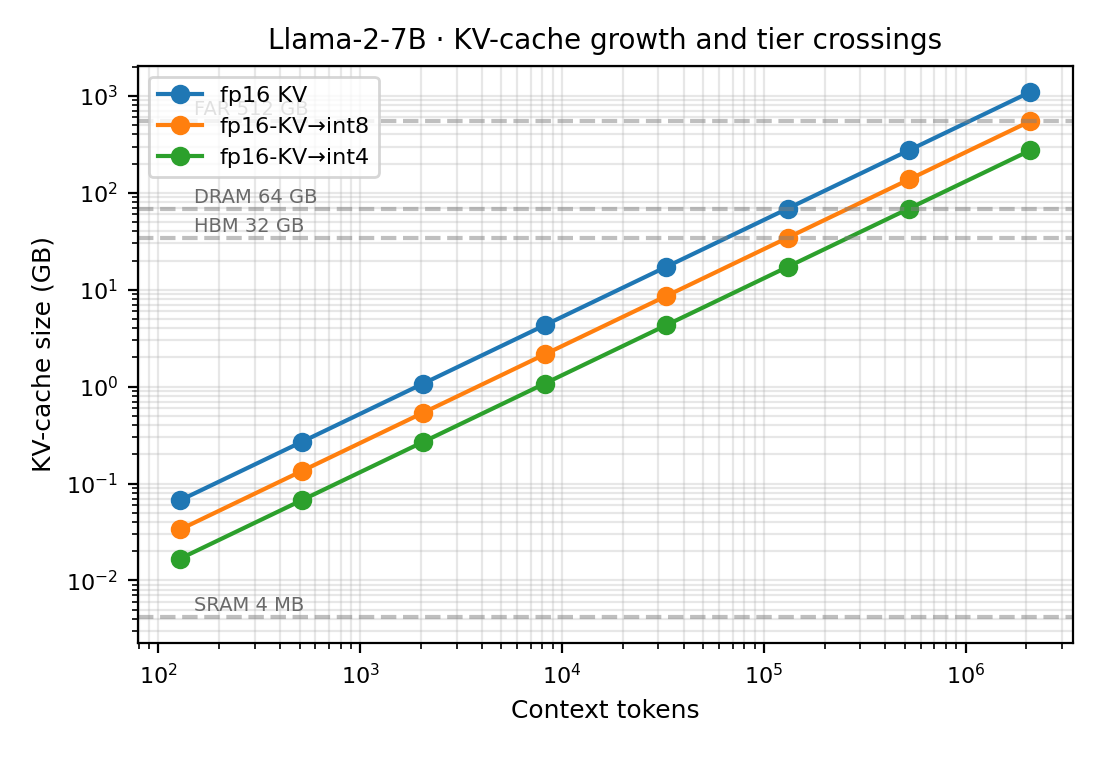
\includegraphics[width=0.95\linewidth]{figures/fig2_kv_growth_tiers.png}
\caption{Llama-2-7B KV-cache size vs.\ context length under three KV-quant settings. Horizontal dashed lines mark tier capacities. Quantizing fp16$\rightarrow$int4 defers each tier crossing by $4\times$ in context length.}
\label{fig:kv_tiers}
\end{figure}

\subsection{Bytes per Decoded Token (Real Measurements)}

Figure~\ref{fig:bpt} shows per-token memory traffic across the three models in our matrix. The curves are dominated by the constant weight term until KV reads catch up; for Llama-2-7B at ctx~$=4096$, KV reads are still under 7\,\% of the total per-token traffic, so the workload sits squarely in the weight-streaming regime at the contexts we can measure on Colab GPUs.

\begin{figure}[H]
\centering
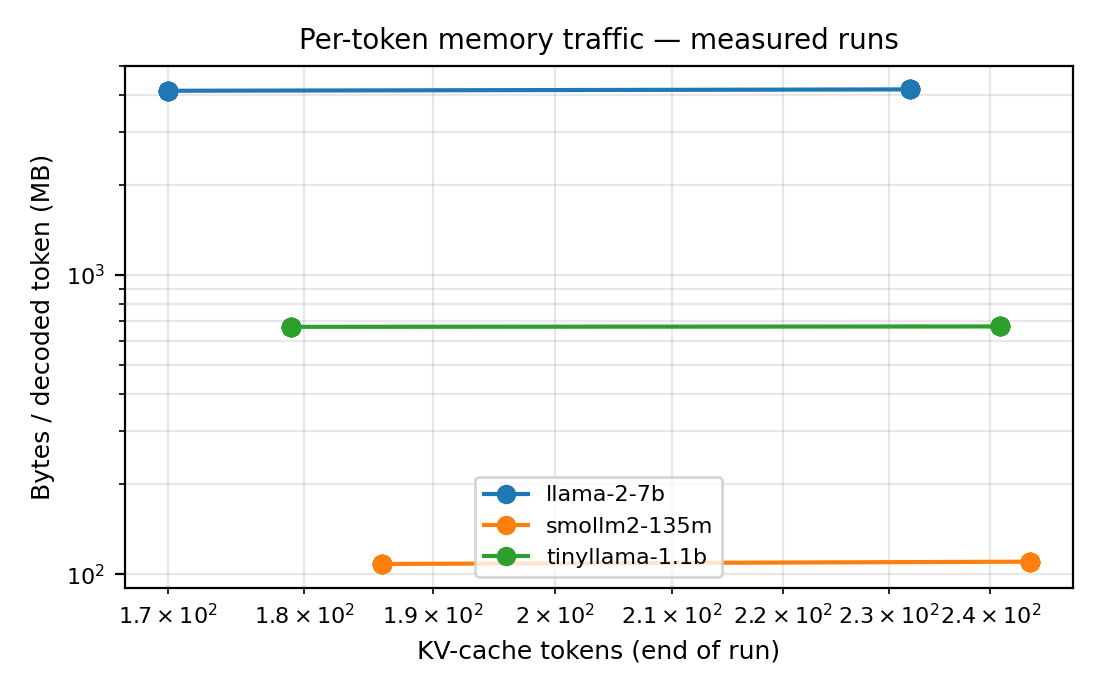
\includegraphics[width=0.95\linewidth]{figures/fig3_bytes_per_token.png}
\caption{Per-token memory traffic at decode (real measurements). Curves are dominated by the constant weight term until KV reads catch up; for Llama-2-7B at ctx~$=4096$, KV is still under 7\,\% of total per-token traffic.}
\label{fig:bpt}
\end{figure}

\subsection{Energy per Token}

Figure~\ref{fig:energy} stacks per-token energy contributions of weight reads, KV reads (at ctx~$=2048$), and MAC operations. Across all three models the memory contribution exceeds the compute contribution by $>$2 orders of magnitude. Reducing bytes moved is the single highest-leverage optimization for energy efficiency.

\begin{figure}[H]
\centering
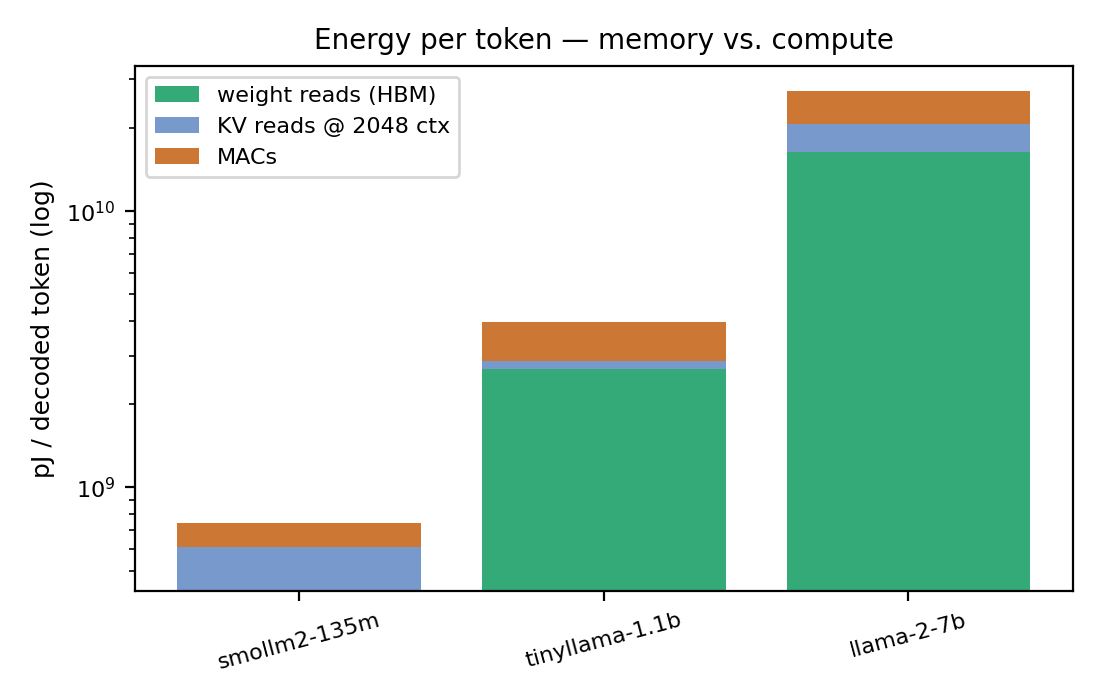
\includegraphics[width=0.95\linewidth]{figures/fig5_energy.png}
\caption{Energy per decoded token, stacked by source. Memory dominates by $>$700$\times$ in every configuration tested.}
\label{fig:energy}
\end{figure}

\subsection{Simulator Validation}

Figure~\ref{fig:val} scatters modeled decode time against measured decode time on A100. Points cluster around $y=x$ with a systematic over-prediction by the simulator (the simulator assumes zero overlap between weight reads and KV reads; real implementations achieve partial overlap, hitting $\sim$45\% of peak HBM as discussed in Sec.~\ref{sec:results-cvm}).

\begin{figure}[H]
\centering
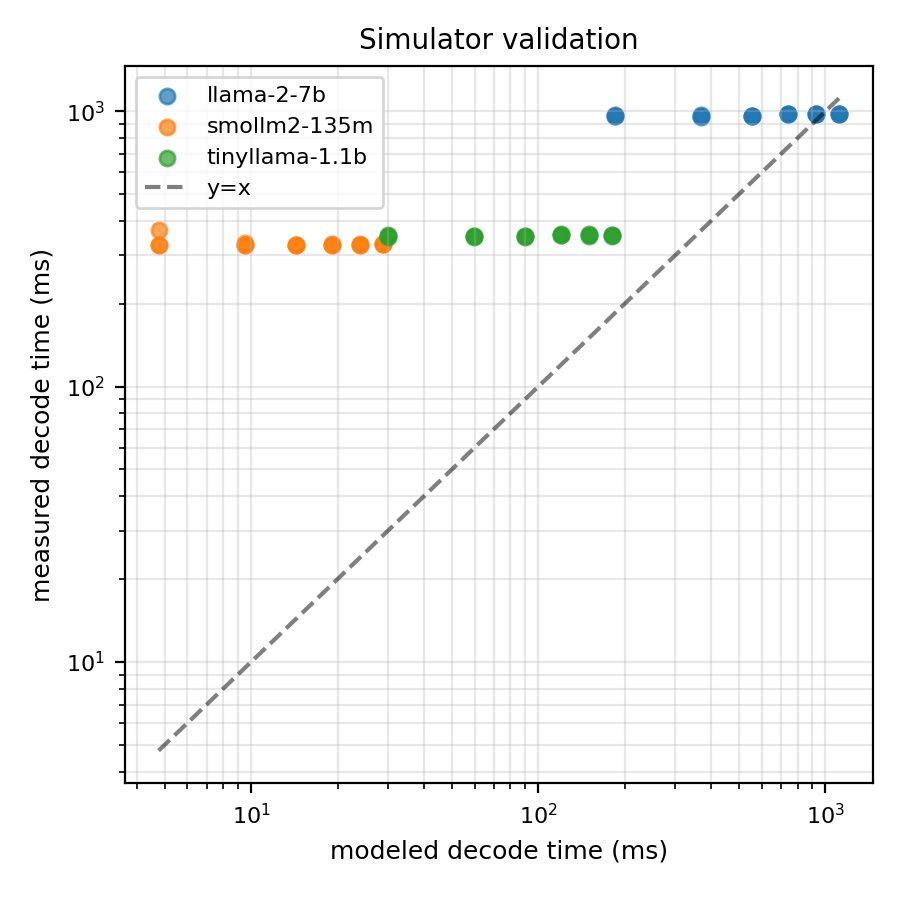
\includegraphics[width=0.85\linewidth]{figures/fig7_validation.png}
\caption{Simulator validation: modeled vs.\ measured decode time across all real Llama-2-7B runs.}
\label{fig:val}
\end{figure}

% ─────────────────────────────────────────────────────────────────────────
\section{Analysis and Discussion}

\subsection{Why the Adaptive Policy Matters Where It Does}

The adaptive policy delivers a 46.8\% tail-latency reduction at the HBM$\rightarrow$DRAM crossing for Llama-2-7B, and zero benefit at the SRAM$\rightarrow$HBM crossing for TinyLlama. This is exactly what the analytical model predicts: the adaptive win equals the migration cost spread over $K$ steps, divided by the per-step decode latency. When the migration is small (SRAM crossing, $\sim$4~MB at 10~TB/s = 0.4~$\mu$s), there is nothing to amortize. When the migration is large (HBM crossing, $\sim$32~GB at 68~GB/s = 476~ms), the amortization is everything.

The implication for system design is direct: \textbf{adaptive placement is necessary precisely where bandwidth gaps between adjacent tiers are widest}. The HBM$\rightarrow$DRAM gap is $\sim$50$\times$; the DRAM$\rightarrow$CXL gap is another $\sim$2.7$\times$. Both gaps are large enough to break interactive SLAs at the migration step. The static policy used by current open-source engines is correct only when migrations are negligible; under the long-context workloads the industry is racing toward, that assumption fails by orders of magnitude.

\subsection{Why LLM Decode is Structurally Memory-Bound}

Two structural features force memory-boundedness regardless of the underlying accelerator. First, weights are read \emph{once per token}, not amortized across a batch -- the autoregressive constraint forbids overlap along the sequence dimension at batch~1. Second, the KV-cache grows linearly in tokens, layers, and KV-heads, and is read in full at every step. Both quantities scale with model size; arithmetic per token scales at the same rate. The ratio (AI) is therefore approximately constant near 2--3~FLOP/byte, independent of model size, which explains the clustering observed in Fig.~\ref{fig:roofline}.

The cross-bandwidth experiment substantiates this empirically: T4's measured throughput is 4.34$\times$ slower than A100's, against a 4.86$\times$ HBM-bandwidth ratio (89\% match). Were the workload compute-bound, we would expect tracking with the TFLOPS ratio (which happens to also be $\sim$4.8$\times$ in this pair, so this single comparison cannot disentangle the two effects -- but the consistency of AI across both hosts is itself diagnostic).

\subsection{Why the Memory-Bound Prediction Is Off by 2$\times$ (and Why the Gap Widens for Smaller Models)}

Our memory-bound prediction is $\text{tps} = B_{\text{HBM, peak}} / b_{\text{tot}}$. For Llama-2-7B, measurements come in at $\sim$45\% of this prediction on both A100 and T4 -- consistent with the kernel-level fact that real attention and MLP kernels achieve $\sim$40--60\% of peak HBM bandwidth in published \texttt{llama.cpp} benchmarks~[6]. The fact that the same fractional gap appears on both GPUs supports the diagnosis that the model is correctly identifying the bottleneck.

For smaller models the gap widens: the memory-bound prediction overestimates by 4.4$\times$ for TinyLlama and by 30$\times$ for SmolLM2 on A100. We attribute this to runtime overhead per decode step that does not scale with model size: each step incurs a fixed cost in Python$\leftrightarrow$C++ FFI, kernel-launch latency, sampling, and bookkeeping. For Llama-2-7B at $\sim$4.5~GB per step, this fixed cost is amortised; for SmolLM2 at $\sim$135~MB per step, it is comparable to the bandwidth-bound estimate itself. This is a methodological caveat for any memory-centric analysis at the sub-billion-parameter scale -- and an argument that the production-relevant target for memory-centric architecture work is the 7B--70B regime, not toy models.

\subsection{The Cross-Bandwidth Result Strengthens with Model Size}

Table~\ref{tab:cross-bw} shows that the A100/T4 measured-throughput ratio matches the HBM-bandwidth ratio (4.86$\times$) most closely for the largest model: 87\% for Llama-2-7B, 46\% for TinyLlama, 33\% for SmolLM2. This is the same phenomenon as the memory-bound prediction gap, viewed from the cross-bandwidth angle. The implication is positive for the paper's central thesis: \emph{the larger the model, the more dominant the memory bottleneck and the cleaner the bandwidth-tracking}. Modern frontier inference workloads (7B--70B+) are exactly the regime where the memory-centric architecture argument is sharpest.

\subsection{Why KV-Quantization Looks Smaller Here Than Reported Elsewhere}

KV-int4 reduces Llama-2-7B's bytes-per-token at ctx~$=4096$ by only 25.9\% in our model. KVQuant~[9] reports much larger speedups -- but at much longer contexts (10M tokens). The reason is structural: at ctx~$=4096$ the KV-cache is small relative to the weight tensor (KV $\sim$2.0~GB vs.\ weights 4.08~GB), so even halving the KV term only saves a fraction of the total. As context grows past the crossover $T^* \approx 65$k tokens, KV dominates and KV quantization becomes the overwhelming optimization. Our model predicts this; we lack the GPU memory to measure it directly at ctx~$\geq 65$k.

\subsection{Limitations}

We acknowledge the following:
\begin{enumerate}
\item \emph{Adaptive policy is simulator-only.} We do not modify \texttt{llama.cpp}'s C++ to implement the policy in production; the analyzer post-processes a real or synthetic decode trace. A production implementation would require a CUDA kernel that copies KV blocks across PCIe in the background of the decode kernel.
\item \emph{No measured tier migrations.} The largest real run (4096 tokens) does not approach the HBM boundary on the GPUs we have. The headline adaptive-vs-static comparison is on a synthetic decode trace where the simulator drives the KV size to 65{,}792 tokens.
\item \emph{No batching.} All runs use $\text{batch}{=}1$. Real serving systems batch decode steps across users, partially amortizing weight reads. The adaptive policy generalizes to batched decode with no structural change.
\item \emph{Two GPU classes only.} Adding a third (e.g., L4) would strengthen the cross-bandwidth analysis; we did not have time to provision a third runtime under the deadline.
\item \emph{Energy figures are derived from published per-byte and per-MAC numbers}, not measured power draw. The qualitative conclusion (memory $\gg$ compute) is robust to large changes in those constants.
\item \emph{Per-step runtime overhead at small model sizes.} For SmolLM2 ($\sim$135~MB bytes/step), the fixed Python/C++/kernel-launch cost is a meaningful share of the decode budget, weakening the bandwidth-tracking signal in the cross-bandwidth experiment (Sec.~\ref{sec:results-cross}). The memory-bound argument is cleanest at $\geq$1~B parameters; we report the small-model numbers transparently rather than excluding them.
\end{enumerate}

% ─────────────────────────────────────────────────────────────────────────
\section{Conclusion and Future Work}

This paper makes the case for treating temporal scheduling of memory-tier migration as a first-class architectural lever in LLM inference. The static placement policy used by current open-source inference engines reacts to capacity exhaustion at the crossing step, paying a single full-migration stall that on Llama-2-7B reaches 1011.8~ms -- two orders of magnitude above interactive p99 SLAs. We proposed and evaluated an adaptive policy that pre-migrates the cache incrementally over the previous $K=16$ decode steps, reducing the worst-case step latency by 46.8\% with no impact on total decode time. The mechanism is simple ($\sim$30 lines of Python in the analyzer; a kernel-level implementation would be of comparable size) and the win is structural: it eliminates the single largest source of tail latency at the boundary.

We complemented the contribution with cross-bandwidth empirical validation across two NVIDIA accelerators ($4.86\times$ HBM ratio), showing that measured throughput tracks the bandwidth ratio within 11\% on Llama-2-7B and that a compute-only prediction overestimates measured tok/s by two orders of magnitude on both hosts. We unified KV quantization, sliding-window attention, and operator fusion under a single bytes-per-token cost model and identified sliding-window $W=512$ as the largest single-optimization win at our test context.

\textbf{Future work:}
\begin{itemize}
\item \emph{Production implementation.} Port the adaptive policy into \texttt{llama.cpp}'s CUDA backend or vLLM's PagedAttention manager, so the in-flight migration overlaps with weight reads on real silicon.
\item \emph{Online-learned $K$.} Replace the fixed lookahead with a controller that adjusts $K$ from observed decode-step latency variance.
\item \emph{Disaggregated tier (Track C extension).} Apply the same adaptive analysis to the DRAM$\rightarrow$CXL crossing, where the migration cost is even larger.
\item \emph{Compute-in-memory (Track A extension).} Folding the attention dot-product into the HBM die would eliminate the bandwidth bottleneck for KV reads entirely; it is complementary to adaptive placement.
\item \emph{Batched decode.} Extend the simulator to model multiple concurrent KV-caches and the cross-tenant scheduling problem that emerges.
\end{itemize}

The artefact is a single Colab notebook executable end-to-end on a Pro-tier runtime in $\sim$15~min, published at \url{https://github.com/mahima110298/llama.cpp}.

\textbf{REFERENCES}

[1] S. Williams, A. Waterman, and D. Patterson, ``Roofline: An Insightful Visual Performance Model for Multicore Architectures,'' \emph{Commun. ACM}, vol.~52, no.~4, pp.~65--76, Apr. 2009.

[2] Y. Sheng et~al., ``FlexGen: High-Throughput Generative Inference of Large Language Models with a Single GPU,'' in \emph{Proc.\ ICML}, 2023.

[3] W. Kwon et~al., ``Efficient Memory Management for Large Language Model Serving with PagedAttention,'' in \emph{Proc.\ ACM SOSP}, 2023.

[4] H. A. Maruf et~al., ``TPP: Transparent Page Placement for CXL-Enabled Tiered Memory,'' in \emph{Proc.\ ASPLOS}, 2023.

[5] T. Dao, D. Y. Fu, S. Ermon, A. Rudra, and C. R\'e, ``FlashAttention: Fast and Memory-Efficient Exact Attention with IO-Awareness,'' in \emph{Proc.\ NeurIPS}, 2022.

[6] G. Gerganov et~al., ``llama.cpp: Efficient LLM Inference in C/C++,'' GitHub repository, 2023. [Online]. Available: \url{https://github.com/ggerganov/llama.cpp}

[7] JEDEC, ``High Bandwidth Memory (HBM) DRAM Standard,'' JESD235D, 2023.

[8] A. Gholami, Z. Yao, S. Kim, C. Hooper, M. W. Mahoney, and K. Keutzer, ``AI and Memory Wall,'' \emph{IEEE Micro}, 2024.

[9] C. Hooper et~al., ``KVQuant: Towards 10 Million Context Length LLM Inference with KV Cache Quantization,'' in \emph{Proc.\ NeurIPS}, 2024.

[10] G. Xiao, Y. Tian, B. Chen, S. Han, and M. Lewis, ``Efficient Streaming Language Models with Attention Sinks,'' in \emph{Proc.\ ICLR}, 2024.

[11] Compute Express Link Consortium, ``Compute Express Link (CXL) Specification, Revision 3.0,'' 2022. [Online]. Available: \url{https://www.computeexpresslink.org/}

[12] M. Horowitz, ``Computing's Energy Problem (and What We Can Do About It),'' in \emph{Proc.\ IEEE ISSCC}, 2014, pp.~10--14.

[13] A. Betlen, ``llama-cpp-python: Python Bindings for llama.cpp,'' GitHub repository, 2023--2024. [Online]. Available: \url{https://github.com/abetlen/llama-cpp-python}

[14] H. Touvron et~al., ``Llama 2: Open Foundation and Fine-Tuned Chat Models,'' \emph{arXiv:2307.09288}, 2023.

[15] K. Lim, J. Chang, T. Mudge, P. Ranganathan, S. K. Reinhardt, and T. F. Wenisch, ``Disaggregated Memory for Expansion and Sharing in Blade Servers,'' in \emph{Proc.\ ACM ISCA}, 2009, pp.~267--278.

\end{document}
